% Template for PLoS
% Version 1.0 January 2009
%
% To compile to pdf, run:
% latex plos.template
% bibtex plos.template
% latex plos.template
% latex plos.template
% dvipdf plos.template

\documentclass[10pt]{article}

% amsmath package, useful for mathematical formulas
\usepackage{amsmath}
% amssymb package, useful for mathematical symbols
\usepackage{amssymb}

% graphicx package, useful for including eps and pdf graphics
% include graphics with the command \includegraphics
\usepackage{graphicx}

% cite package, to clean up citations in the main text. Do not remove.
\usepackage{cite}

\usepackage{color} 

% Use doublespacing - comment out for single spacing
%\usepackage{setspace} 
%\doublespacing


% Text layout
\topmargin 0.0cm
\oddsidemargin 0.5cm
\evensidemargin 0.5cm
\textwidth 16cm 
\textheight 21cm

% Bold the 'Figure #' in the caption and separate it with a period
% Captions will be left justified
\usepackage[labelfont=bf,labelsep=period,justification=raggedright]{caption}

% Use the PLoS provided bibtex style
\bibliographystyle{plos}

% Remove brackets from numbering in List of References
\makeatletter
\renewcommand{\@biblabel}[1]{\quad#1.}
\makeatother


% Leave date blank
\date{}

\pagestyle{myheadings}
%% ** EDIT HERE **


%% ** EDIT HERE **
%% PLEASE INCLUDE ALL MACROS BELOW
\newcommand{\citep}[1]{\cite{#1}} %natbib compatibility
\newcommand{\citet}[1]{\cite{#1}}
\newcommand{\de}{$^\circ$~} 
%% END MACROS SECTION

\begin{document}

% Title must be 150 characters or less
\begin{flushleft}
{\Large
\textbf{Lattice Spacing and Multi-dimensional Forces in the Cross-bridge}
}
% Insert Author names, affiliations and corresponding author email.
\\
C.\ David Williams$^{1,\ast}$, 
Michael Regnier$^{2}$, 
Thomas L.\ Daniel$^{3}$
\\
\bf{1} Department of Physiology and Biophysics, University of Washington, Seattle, Washington, United States of America
\\
\bf{2} Department of Bioengineering, University of Washington, Seattle, Washington, United States of America
\\
\bf{3} Department of Biology, University of Washington, Seattle, Washington, United States of America
\\
$\ast$ E-mail: cdave@uw.edu
\end{flushleft}

% Please keep the abstract between 250 and 300 words
\section*{Abstract}
Existing mechanochemical models of muscle contraction treat myosin as a simple linear spring arranged parallel to the contractile filaments.
These single-spring models cannot simulate the radial force that muscle generates (orthogonal to the direction of contraction) or the effects of altered filament lattice spacing. 
We describe a more complex myosin cross-bridge model that uses multiple springs to replicate myosin's force-generating power stroke and account for the effects of lattice spacing and radial force. 
The four springs which comprise this model (the 4sXB) correspond to the mechanically relevant portions of myosin's structure.
As occurs \emph{in vivo}, the 4sXB's state-transition kinetics and force production dynamics vary with lattice spacing.

Additionally, we describe a simpler two spring cross-bridge (2sXB) model which produces results similar to those of the 4sXB model.
Unlike the 4sXB model, the 2sXB model requires no iterative techniques, making it more computationally efficient.
The rate at which the multi-spring cross-bridges bind and generate force decreases as lattice spacing grows. 
Axial and radial forces generated by the 4sXB and 2sXB increase in magnitude as lattice spacing is offset from the myosin head resting position. 
Importantly, our results mirror those for intact, contracting muscle force production.

\emph{Keywords:} cross-bridge model; cross-bridge kinetics; lattice spacing; radial force; muscle model; myosin 

% Please keep the Author Summary between 150 and 200 words
% Use first person. PLoS ONE authors please skip this step. 
% Author Summary not valid for PLoS ONE submissions.   
\section*{Author Summary}
Models of muscle contraction have long treated the molecular motor myosin as a simple spring oriented parallel to its direction of movement. 
This assumption does not allow prediction of some forces observed during muscle shortening, or for a description of the relationship between the maximum force produced and the spacing between contractile filaments. 
We develop an alternative model, still computationally efficient enough to be used in simulations of the sarcomere, that incorporates both linear and torsional (angle dependent, like those found in a watch) springs. 
This new type of model captures much of the behavior missing from single-spring models of the cross-bridge.


\section*{Introduction}
Radial forces are of the same order as axial forces in contracting muscles \citep{Maughan1981, Cecchi1990, Millman1998}. 
These forces, along with the radial lattice spacing of myofilaments, are thought to be key determinants of muscle force generation \citep{Fuchs2005}. 
At the same time, structural information about myosin cross-bridges suggests that force is generated through the action of a lever arm \citep{Rayment1993, Uyeda1996, Huxley2000}.
That lever arm generates the strain accompanying the power stroke via a change in the rest angle at which the lever is attached to S1 region \citep{Huxley2000, Houdusse2001}. 
This change in angle occurs at the converter region, a flexible area which acts as a torsional spring. 
These phenomena may be related: the radial forces a cross-bridge generates are a result of the lever arm's geometry \citep{Schoenberg1980b}. 

Existing theoretical and computational models of cross-bridge force generation, at the level of myofilaments, assume force is generated by a simple linear spring oriented parallel to the long axis of the myofilaments (Fig.~\ref{fig_xb_types}B). 
This assumption has persisted from the earliest fundamental models of muscle contraction to more elaborate and spatially explicit models \citep{Huxley1957, Daniel1998, Chase2004, Tanner2007, Campbell2009}.  
These single-spring models have yielded insight into the processes that regulate production of force in the direction of contraction.
However, these prior models of muscle contraction have paid less attention to radial forces and the effects of changes in filament lattice spacing. 
As a result, geometries of the single spring cross-bridge models have changed little while kinetic schemes governing transitions between conformational states have increased in complexity \citep{Huxley1957, Pate1989, Daniel1998, Smith2008a}. 
To analyze the radial forces that occur during muscle contraction, a different cross-bridge geometry is needed: a geometry that produces both forces aligned with and forces orthogonal to the direction of contraction. 
A lever arm made of several springs can simulate the deformations a cross-bridge undergoes as it generates force (the power stroke), can provide a geometry which is usable in cross-bridge models, and can account for both axial and radial forces \citep{Houdusse2001}.  

Here we detail two models of cross-bridges that use multiple springs to replicate the lever arm mechanism and capture its biologically relevant effects.  
Both are affected by changes in lattice spacing and account for the radial component of force produced during the power stroke.  
The first model (referred to as the 4sXB model) simulates the cross-bridge as a system of four linearly elastic springs arranged in a geometry based upon the structure of the S1 and S2 regions of myosin II (Fig.~\ref{fig_xb_types}D).  
Our second model (referred to as the 2sXB model) consists of two linearly elastic springs and provides greater computational efficiency than the 4sXB model while replicating many of the more complex model's behaviors (Fig.~\ref{fig_xb_types}C). 
Both the 4sXB model and the 2sXB model use a three-state model of the cross-bridge cycle's kinetics, consisting of an unbound state, a low-force pre-power stroke state, and a force-producing post-power stroke state. 
The kinetics of transition from one state to another in our models are similar to those used previously but are generalized for use in two dimensions; our kinetics calculate transition probabilities using the free energy landscape of the cross-bridges instead of the offset of the cross-bridge head (Fig.~\ref{fig_xb_types}A) \citep{Pate1989, Daniel1998, Takagi2004, Tanner2007}. 
We quantify both axial and the radial forces produced by our two cross-bridge models. 
Additionally, we explain how changes in lattice spacing affect kinetics and forces in our multiple-spring models. 

% Results and Discussion can be combined.
\section*{Results}

\subsection*{Subsection 1}

\subsection*{Subsection 2}

\section*{Discussion}

% You may title this section "Methods" or "Models". 
% "Models" is not a valid title for PLoS ONE authors. However, PLoS ONE
% authors may use "Analysis" 
\section*{Materials and Methods}

% Do NOT remove this, even if you are not including acknowledgments
\section*{Acknowledgments}


%\section*{References}
% The bibtex filename
\bibliography{JournalArticles,NotArticles}

\clearpage
\section*{Figure Legends}
\begin{figure}[ht]
    \begin{center}
    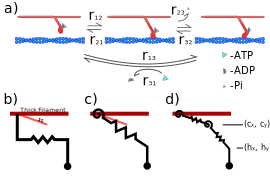
\includegraphics[width=3.2in]{../imgs/Figure1.pdf}
    \caption{ \textbf{Kinetics and cross-bridge types.} 
        (A)  The three state kinetic system. 
        The three states represent (1) an unbound state, (2) a pre-power stroke state, and (3) a post-power stroke state. 
        The rate of transition between states $i$ and $j$ is represented as $r_{ij}$. 
        The forward and reverse transition rates are functions of energy stored in the cross-bridge. 
        (B)--(D) The three cross-bridge models, plotted against a myosin crystal structure for comparison (structure image generated from \protect\citet{Gourinath2003} with PyMol \protect\citep{pymol}).
        The energy landscape of each cross-bridge and the free energy at rest lattice spacing are shown adjacent to the cross-bridge schematic.
        (B) The 1sXB introduced in \protect\citep{Huxley1957}. 
        (C) The 2sXB which uses a torsional/angular spring ($\theta$) and a linear spring ($\rho$). 
        (D) The 4sXB with two torsional and two linear springs.
        Of the 4sXB's springs, $\alpha$ corresponds to the point at which the S2 region rejoins the thick filament backbone, $\beta$ to the S2 region itself, $\gamma$ to the area linking the S2 and the light chain domains, and $\delta$ to the light chain domain itself.
        It is $\gamma$ that replicates the change in angle accompanying the powerstroke.
        \label{fig_xb_types}
        }
    \end{center}
\end{figure}

\begin{figure}[ht]
    \begin{center}
    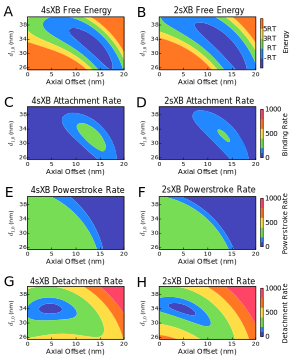
\includegraphics[width=3.25in]{../imgs/Figure2.pdf}
    \caption{ \textbf{Energy and kinetics of the multi-spring cross-bridge models as a result of changes to axial offset and lattice spacing.} 
        Axial offset is the distance between the current axial location of the cross-bridge's tip and the location where the cross-bridge attaches to the thick filament.  
        Lattice spacing ($d_{10}$) is defined as in \protect\citet{Millman1998}, with an offset to account for filament thicknesses so the cross-bridge spans the filaments at a rest lattice spacing of 34 nm. 
        (A)--(H)  The properties of the 4sXB model (A, C, E, and G) and the 2sXB model (B, D, F, and H) as they change with binding site offset and lattice spacing.
        (A) depicts the free energy of the 4sXB model at various lattice spacings, with the head stretched to an axial offset from the thick filament attachment point.
        The free energy of the 2sXB model is shown in (B).  
        (C) and (D) show $r_{12}$, the probability that the 4sXB and 2sXB models will transition from an unbound state to a bound state. 
        (E) and (F) show $r_{23}$, the probability of transition from a pre-power stroke state to a post-power stroke state, for the same cross-bridges, axes, and scales as (C) and (D) show $r_{12}$.
        (G) and (H) show $r_{31}$, the probability of unbinding from a post-power stroke state. 
        The reverse rates, $r_{21}$, $r_{32}$, and $r_{13}$ are back-calculated from the forward rates.
        \label{fig_kinetics_contours}
        }
    \end{center}
\end{figure}

\begin{figure}[ht]
    \begin{center}
    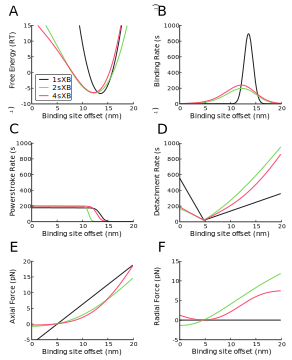
\includegraphics[width=3.25in]{../imgs/Figure3.pdf}
    \caption{ \textbf{Forces, energy, and kinetics of the 1sXB, 2sXB, and 4sXB models at resting lattice spacing.}
        (A)--(F) show the energy, transition rates, and forces of the 1sXB model (black), 2sXB model (green), and 4sXB model (red) at resting lattice spacing.  
        The 1sXB model values shown for comparison are derived from those of \protect\citet{Daniel1998} and \protect\citet{Tanner2007}, shifted axially so the resting location of the cross-bridge head in each case is aligned with the resting locations of the 2sXB model and 4sXB model allowing easier comparison. 
        The free energy of the cross-bridges in state two is shown in (A), where the multi-spring cross-bridges' shifts from a strictly parabolic trajectory is visible. 
        The explicit two-dimensional thermal forcing of the multi-spring cross-bridge heads in (B) results in binding probabilities that are more distributed than those of the single spring cross-bridge.
        The rate of power strokes (C) remains least changed between the single and the multi-spring cross-bridge models.  
        The energy-based kinetics of the multi-spring cross-bridges are unable to fully replicate the biased detachment rate of the 1sXB model in (D).
        (E) and (F) show the 1sXB's sharp discontinuities in axial force and lack of any radial force.
        \label{fig_kinetics_cuts}
        }
    \end{center}
\end{figure}

\
\begin{figure}[ht]
    \begin{center}
    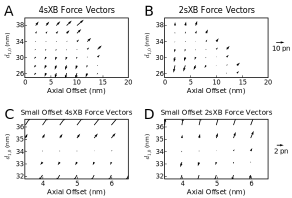
\includegraphics[width=3.25in]{../imgs/Figure4.pdf}
    \caption{ \textbf{Overview and detail of the forces exerted by the 2sXB and 4sXB\@ models.}
        (A)--(D) show the forces exerted by the 4sXB and the 2sXB models; omitted are vectors for unlikely configurations as determined by the sum of $r_{23}$ and the inverse of $r_{31}$. 
        (A) and (B) show overviews of the forces exerted, respectively, by the 4sXB model and the 2sXB model over lattice spacings and axial offsets that vary as in Figure 2. 
        The forces exerted by the two cross-bridges have radial components which frequently equal or exceed their axial components. 
        A more detailed view of the region surrounding the rest position of the cross-bridges is shown in (C) and (D), where the large radial components of the cross-bridge forces, particularly for the 2sXB model, is again evident.  (E)--(H) show, separated, the axial and radial components of the 4sXB and the 2sXB models.
        \label{fig_forces}
        }
    \end{center}
\end{figure}

\
\begin{figure}[ht]
    \begin{center}
    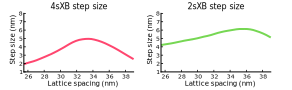
\includegraphics[width=3.25in]{../imgs/FigureS1.pdf}
    \caption{ \textbf{Changes in step size with lattice spacing.}
        Step size varies as lattice spacing diverges from its rest value.
        Step size is defined as the change in the rest axial offset between the pre- and post-power stroke states. 
        The 4sXB model and 2sXB model exhibit different tuning curves.
        \label{fig_step_size}
        }
    \end{center}
\end{figure}


%\begin{figure}[!ht]
%\begin{center}
%%\includegraphics[width=4in]{figure_name.2.eps}
%\end{center}
%\caption{
%{\bf Bold the first sentence.}  Rest of figure 2  caption.  Caption 
%should be left justified, as specified by the options to the caption 
%package.
%}
%\label{Figure_label}
%\end{figure}


\clearpage
\section*{Tables}
\begin{table}[ht]
    \begin{center}
    \begin{tabular}[t]{|l|ccc|} \hline
    \multicolumn{4}{|l|}{\textbf{4sXB}} \\ 
    \multicolumn{1}{|l}{~} 
              & Rest value & $E$        & Source \\ \cline{2-4}  
    $\alpha$  & 40\de      & 100 pN/rad & \citet{Liu2006}      \\
    $\beta$   & 10.5 nm    & 10 pN/nm   & \citet{Liu2006}      \\
    $\delta$  & 125\de     & 40 pN/rad  & \citet{Taylor1999}   \\
    $\delta'$ & 70\de      & 40 pN/rad  & \citet{Taylor1999}   \\
    $\gamma$  & 9.6 nm     & 5 pN/nm    & \citet{Houdusse2000} \\ \hline
    \multicolumn{4}{|l|}{\textbf{2sXB}} \\ 
    \multicolumn{1}{|l}{~} 
              & Rest value & $E$        & Source      \\ \cline{2-4} 
    $\theta$  & 47\de      & 40 pN/rad  & See caption \\
    $\theta'$ & 73\de      & 40 pN/rad  & See caption \\
    $\rho$    & 20 nm      & 2 pN/nm    & See caption \\
    $\rho'$   & 16 nm      & 2 pN/nm    & See caption \\ \hline
    \end{tabular}
    \caption{ 
	    \label{parameter_table}
	    \textbf{Model parameters and their sources} 
	    Prime values, such as $\delta'$, represent post-power stroke state values. 
	    From \citet{Liu2006}, which used insect flight muscle, the most frequently occurring thick filament to S2 angle range is 51-60\de. 
	    We assume that this range is being distorted by the compressive radial force being generated by the rigor cross-bridges in the swollen lattice spacings that \citet{Liu2006} used. 
	    As such, we choose a rest angle for $\alpha$ at the low end of the still common range of 50\de to 40\de. 
	    We do not change this angle between states one, two and three.
	    In \citet{Taylor1999} (clearly explained in \citet{Davis2009}) the angle between the LCD and the thick filament's axial axis goes from 125\de to 70\de with the power stroke. 
	    The LCD rest length generated by measurements made of structure 1DFK from \citet{Houdusse2000}. 
	    The rest values of the 2sXB model's springs are determined by those of the 4sXB model; they are calculated so that the rest position of the 2sXB's head is the same as the rest position of the 4sXB's head. 
	    The spring constant, $E$, for the angular spring responsible for each cross-bridge's power stroke is determined by the change in angle over the power stroke and the energy liberated by the hydrolysis of ATP \citep{Tanner2007}. 
	    Additional spring constants are chosen to be consistent with previous work, and to provide sufficient flexibility to enable diffusion. 
    }
    \end{center}
\end{table}

%\begin{table}[!ht]
%\caption{
%\bf{Table title}}
%\begin{tabular}{|c|c|c|}
%table information
%\end{tabular}
%\begin{flushleft}Table caption
%\end{flushleft}
%\label{tab:label}
% \end{table}

\end{document}

